\subsection{Results}\label{sec:m1:results}

\subsubsection{Tests}\label{sec:m1:results:tests}
    \cref{fig:m1:omega_tests} show the evolution of the density fractions with time. They sum to one across all times which was required. At early times the radiation density dominates (orange line). The intersection between the orange and green lines mark the radiation-matter equality, after which matter is the dominating density. Likewise, the intersection between the green and purple lines mark the matter-dark energy equality, where dark energy (manifested in the cosmological constant) become the dominating density. Time can thus be divided into three regimes; radiation dominated, matter dominated, and dark energy dominated eras. 
    \begin{figure}
        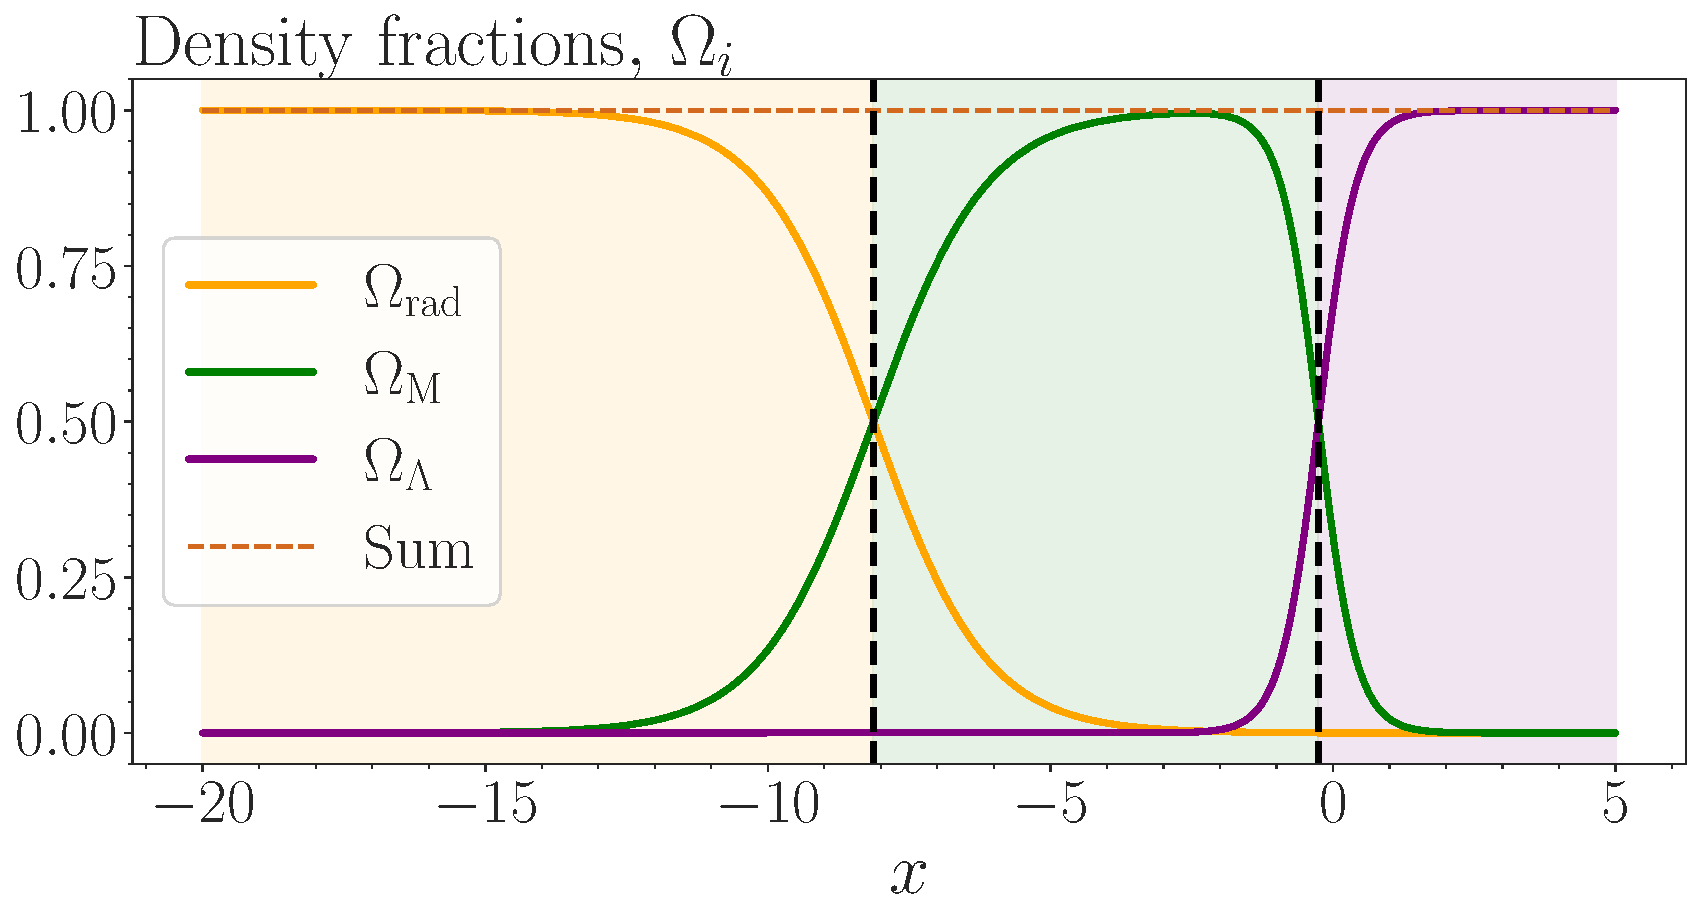
\includegraphics[width=\linewidth]{testing_omegas.pdf}
        \caption{Density fractions $\O_i$ as function of $x$. For low $x$, radiation dominates, before matter dominates and dark has just become the dominant energy density today $x=0$, and will continue to dominate into the future. The sum of densities sums to one across all times, as required.}
        \label{fig:m1:omega_tests}
    \end{figure}

    As explained in section \cref{sec:m1:theory:sanity}, we have analytical solutions for constructions of $\eta$ and $\Hp$ in the different regimes. \cref{fig:m1:eta_tests} is the sanity check for $\eta$, showing $\eta\Hp/c$ converging to finite values in the radiation and matter dominated eras (where $\alpha_{\mathrm{rad}, \mathrm{M}}>0$), and diverging towards $+\infty$ in the dark energy dominated era ($\alpha_\Lambda =-2 <0$). This is in accordance with the analytical solutions. The different regimes are shown in shaded colour. It is also worth noticing that $(\d \eta /\d x)\Hp/c$ is one for all regimes, as expected from equation \cref{eq:m1:theory:measures:eta_diffeq}.

    \begin{figure}
        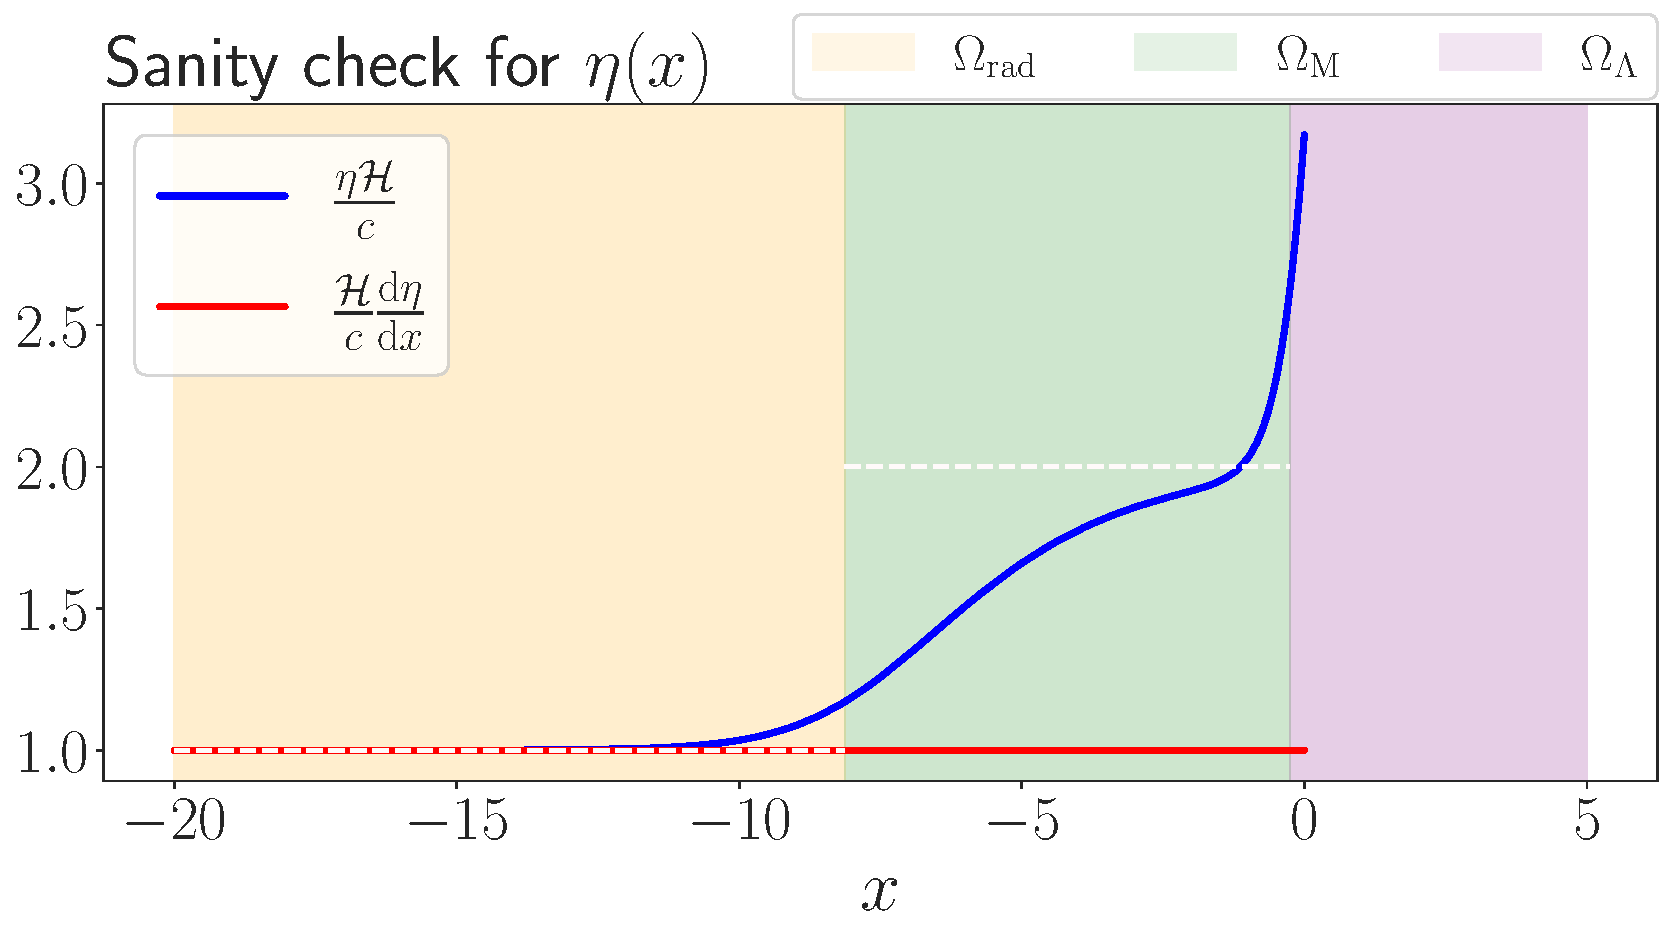
\includegraphics[width=\linewidth]{eta_test.pdf}
        \caption{Sanity check for $\eta$. $\eta\Hp/c$, in blue, is one in the radiation regime, two in the matter regime and diverging toward $+\infty$ in the dark energy regime, as expected from the analytical approximations in each regime. $(\d \eta /\d x)\Hp/c$, in green, is one throughout time, as expected from the differential equation for $\eta$.}
        \label{fig:m1:eta_tests}
    \end{figure}

    \cref{fig:m1:Hp_tests} is the sanity check confirming that our constructions of $\Hp$ and its derivatives converge to the analytical approximation in the different regimes. The second derivative, as shown in blue, takes the value of one in the radiation regime, one half in the matter regime and one in the dark energy regime. Similarly, the first derivative, as shown in green, take the value negative one in the radiation regime, negative one half in the matter regime and one in the dark energy regime. This is well in accordance with the analytical approximations put forth in section \cref{sec:m1:theory:sanity}. 

    \begin{figure}
        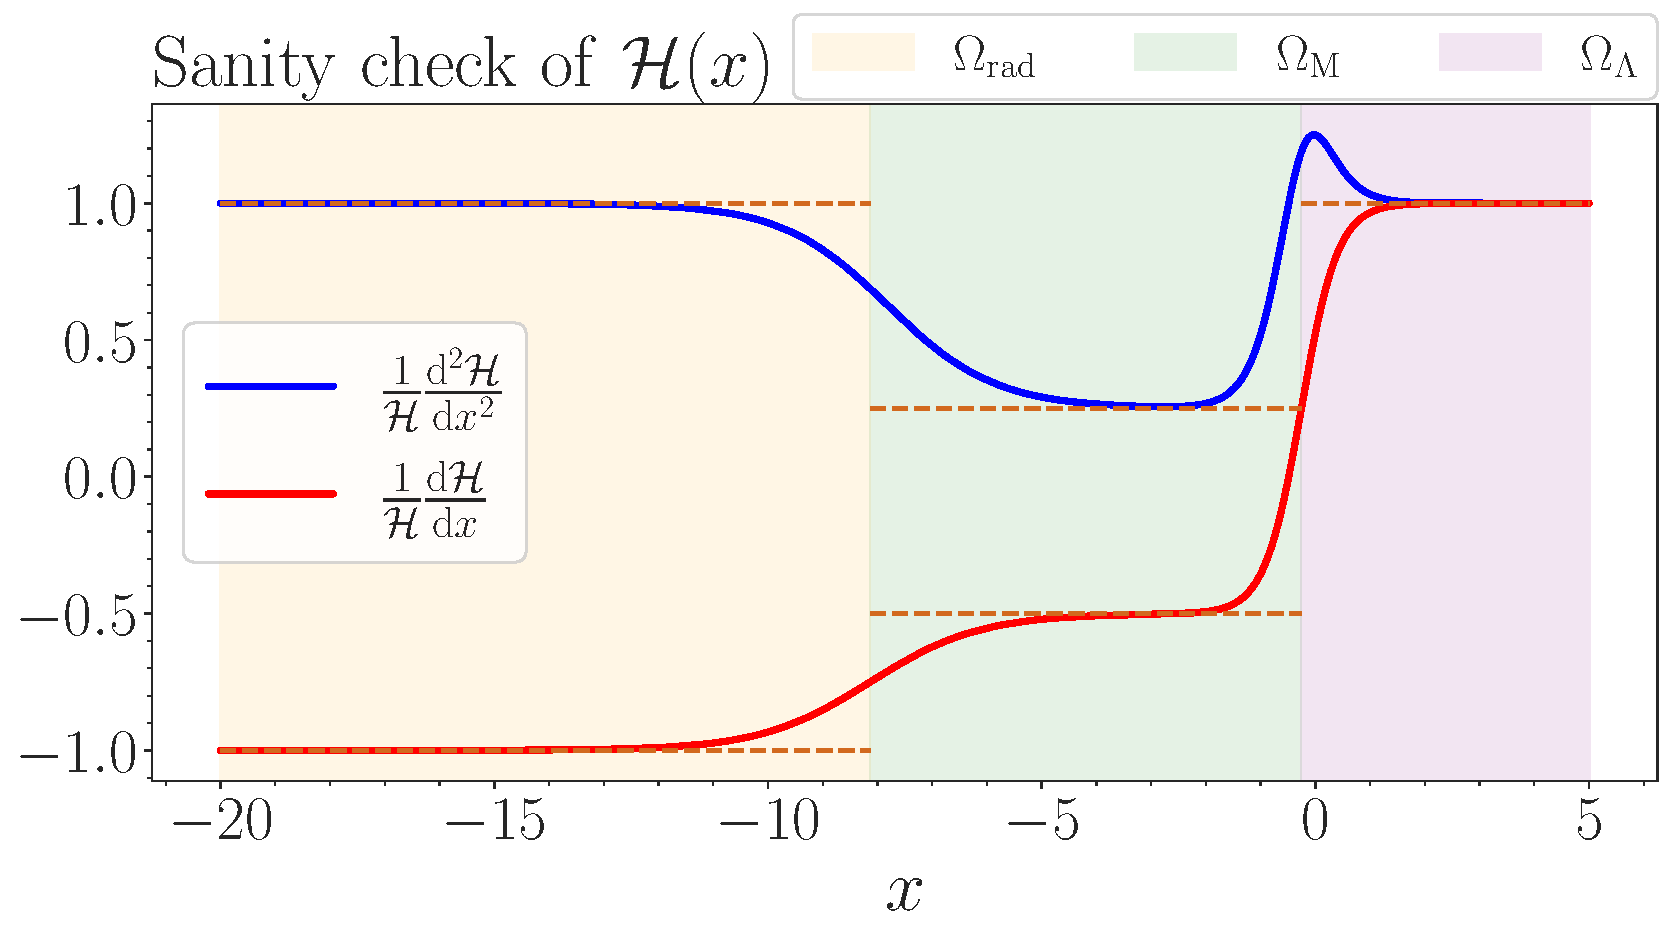
\includegraphics[width=\linewidth]{Hp_test.pdf}
        \caption{Sanity check for $\Hp$, showing that the second derivative (blue) converge to one, one half, and one in the radiation, matter and dark energy regimes respectively. The first derivative (green) converge to negative one, negative one half and one in the same regimes, which are shown as a shaded background.}
        \label{fig:m1:Hp_tests}
    \end{figure}

    These sanity checks are confirmations that the implementation of the model yields the same result as the analytical approximation in the different regimes for various constructions of $\eta$ and $\Hp$ and their derivatives.
    
\subsubsection{Analysis}

    \cref{sec:m1:theory:equalities} indicate how we can calculate the radiation-matter equality (RM-equality), matter-dark energy equality (ML-equality), when the acceleration of the universe started, the age of the universe and the conformal time today. The result is shown in \cref{tab:m1:important_values}. We note that the equalities is in accordance with the sanity checks, and the age of the universe today (in cosmic time) is about 13.9 Gyr. 
    \begin{table}
        \begin{tabular}{lrrrl}
Quantity & x & z & t [Gyr] &  \\
RM-equality  & -8.13 & 3400.33 & 0.000051 &   \\
ML-equality  & -0.26 & 0.29 & 10.378200 &   \\
Accel. start  & -0.26 & 0.29 & 10.378200 &    \\
Age of universe  & 0.00 & 0.00 & 13.857700 &   \\
Conformal time  & 0.00 & 0.00 & 46.318700 &   \\
\end{tabular}

        \caption{Important quantities in the evolution of the universe.}
        \label{tab:m1:important_values}
    \end{table}

    The conformal Hubble factor, $\Hp$, is plotted against time, $x$, in \cref{fig:m1:conformal_hubble_factor_Hp}. It is decreasing in the radiation and matter regimes and increasing in the dark energy regime. Since this is a measure of the expansion of the universe, the acceleration seem to coincide with the matter-dark energy equality. 
    \begin{figure}
        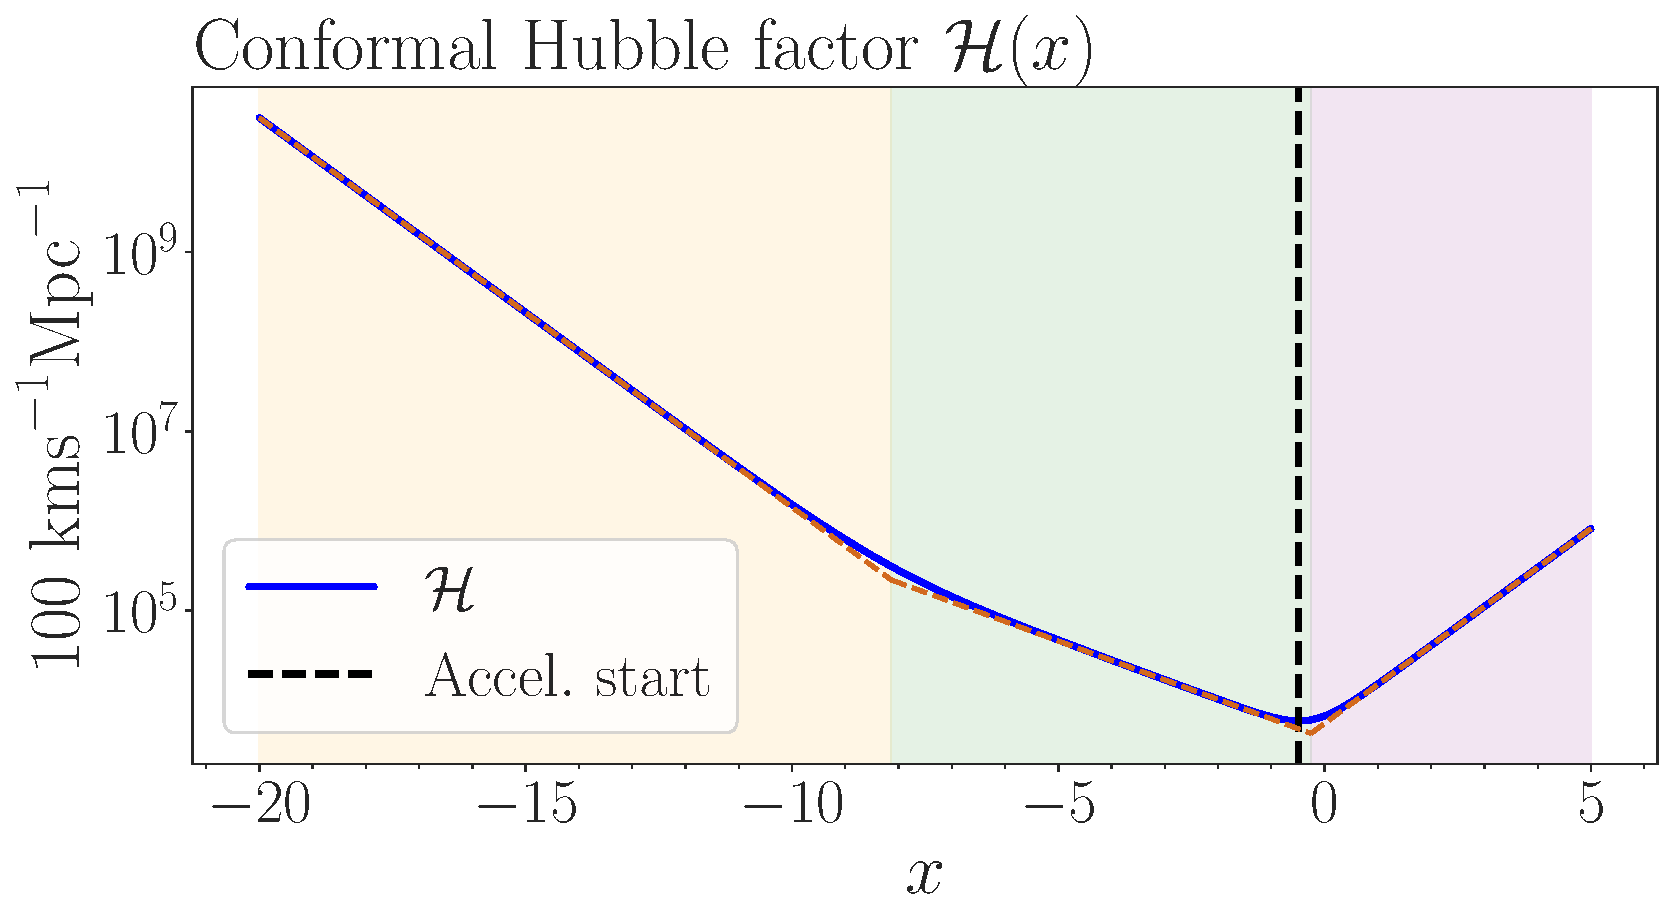
\includegraphics[width=\linewidth]{conformal_hubble_factor.pdf}
        \caption{$\Hp$ as function of $x$. It is decreasing in the radiation and matter regimes, and increasing in the dark energy regime.}
        \label{fig:m1:conformal_hubble_factor_Hp}
    \end{figure}

    \cref{fig:m1:cosmic_conformal_time} show the cosmic time $t$ and the conformal time $\eta/c$. We observe that the cosmic time accelerates around matter-dark energy equality, and seems to diverge, whereas the conformal time increases in the matter regime and seem to converge in the dark energy regime.

    \begin{figure}
        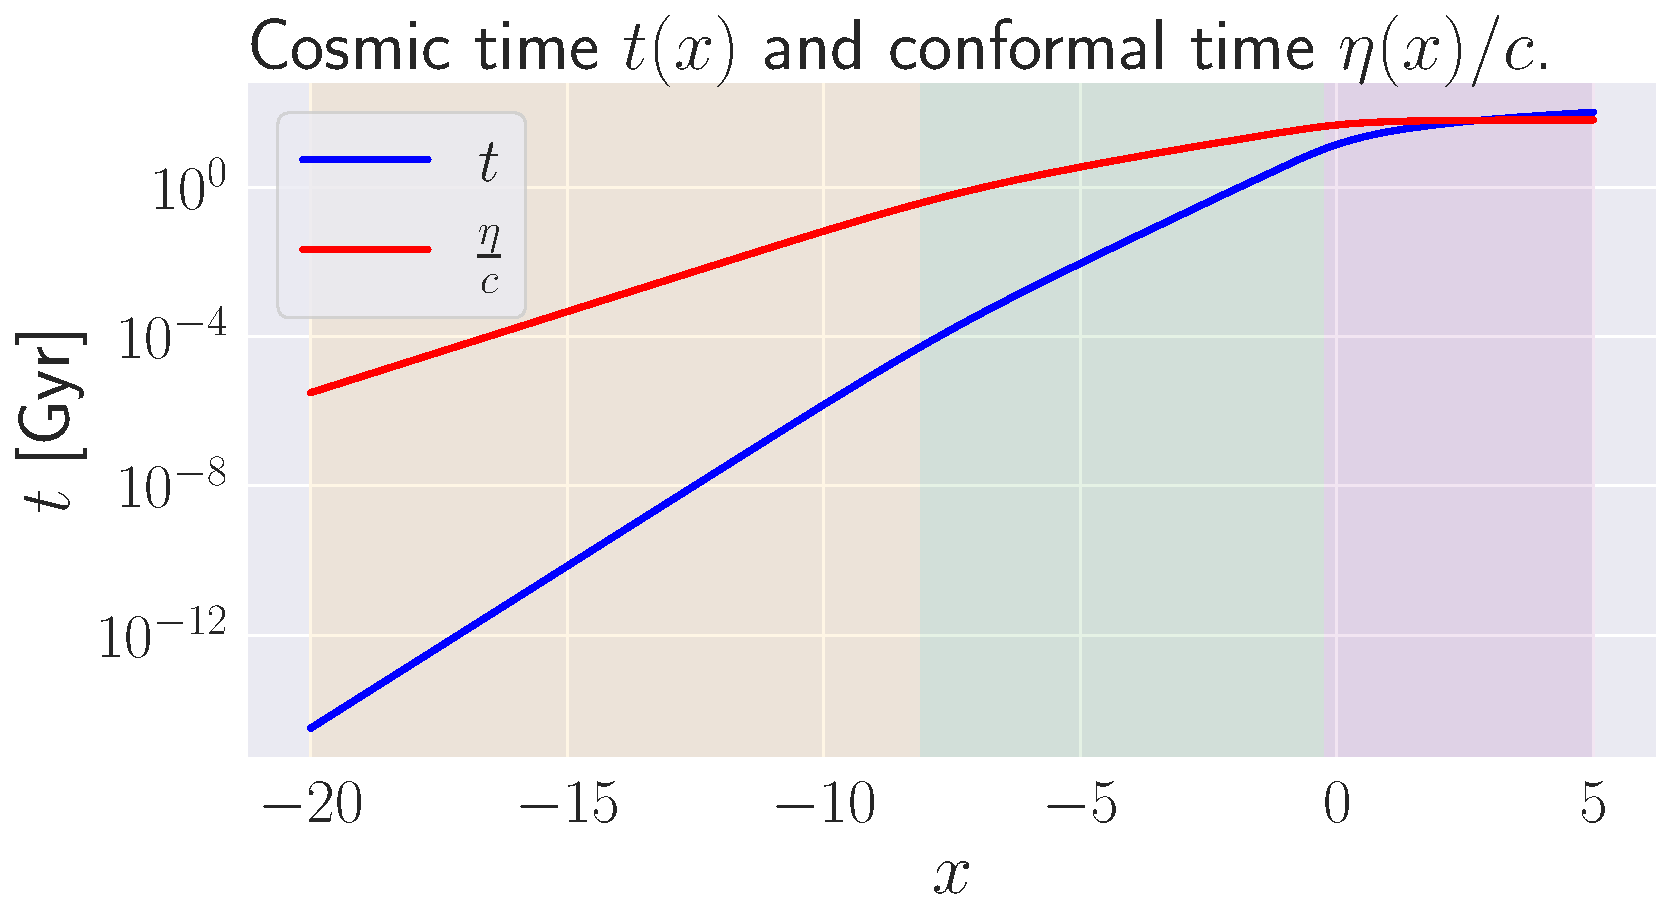
\includegraphics[width=\linewidth]{cosmic_conformal_time.pdf}
        \caption{Cosmic time (in blue) and conformal time (green). Cosmic times increase drastically in the dark energy regime showing a seemingly divergent behaviour. Conformal time increased in the matter regime and seem to converge in the dark energy regime.}
        \label{fig:m1:cosmic_conformal_time}
    \end{figure}

    \cref{fig:m1:supernova_data} shows the supernova data as blue error bars, with the theoretical prediction plotted above it. The quantity plotted is the luminosity distance divided by redshift, $d_L/z$ for better comparison. We notice the accordance between the two, and also note that the $x$-axis in this plot is the redshift $z$ instead of the logarithm of the scale factor. This means that earlier times are to the right in the plot (high redshift), as opposed to the other plots. 

    \begin{figure}
        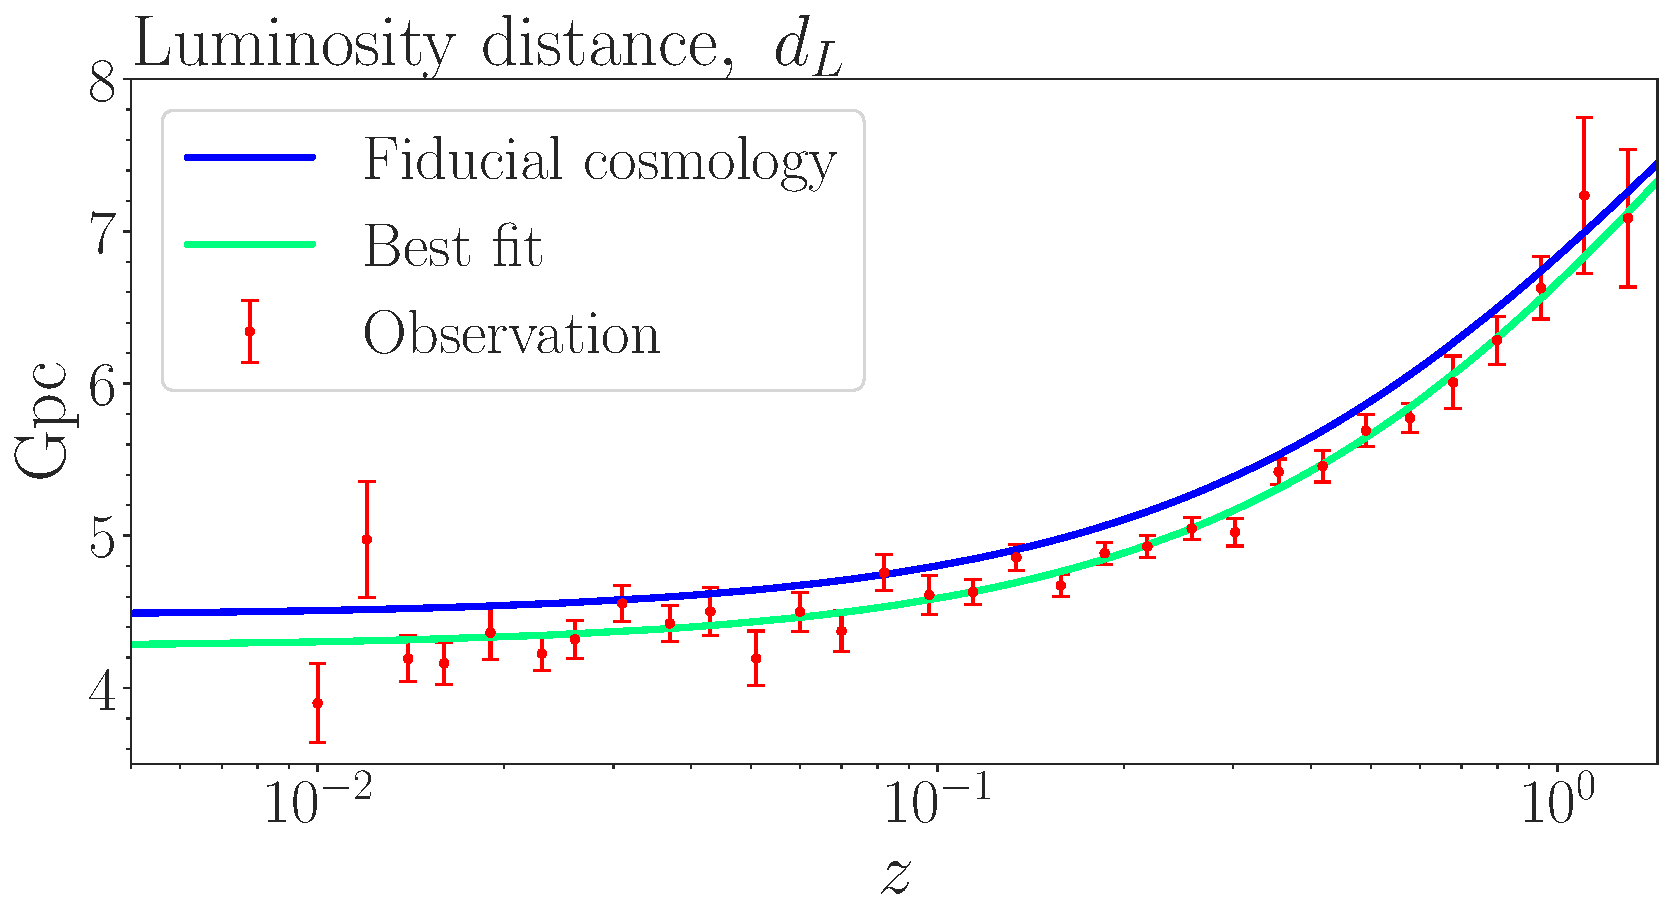
\includegraphics[width=\linewidth]{supernova_data.pdf}
        \caption{Luminosity distance from supernova data shown in blue, and the prediction from the model in green. Notice the $x$-axis is now the redshift $z=e^x-1$.}
        \label{fig:m1:supernova_data}
    \end{figure}

    \cref{fig:m1:omega_planes} shows the $\chi^2$-values found from \cref{eq:m1:chi2_test_def}, to 1$\sigma$ accuracy. The black dotted line represent a flat universe, where the matter and dark energy are the main constituents of the universe. The supernova data originate in close temporal proximity to us, we thus assume that the contribution from the radiation density is negligible for making constraints on $\O_\mathrm{M}$ and $\O_\Lambda$ today. 

    \begin{figure}
        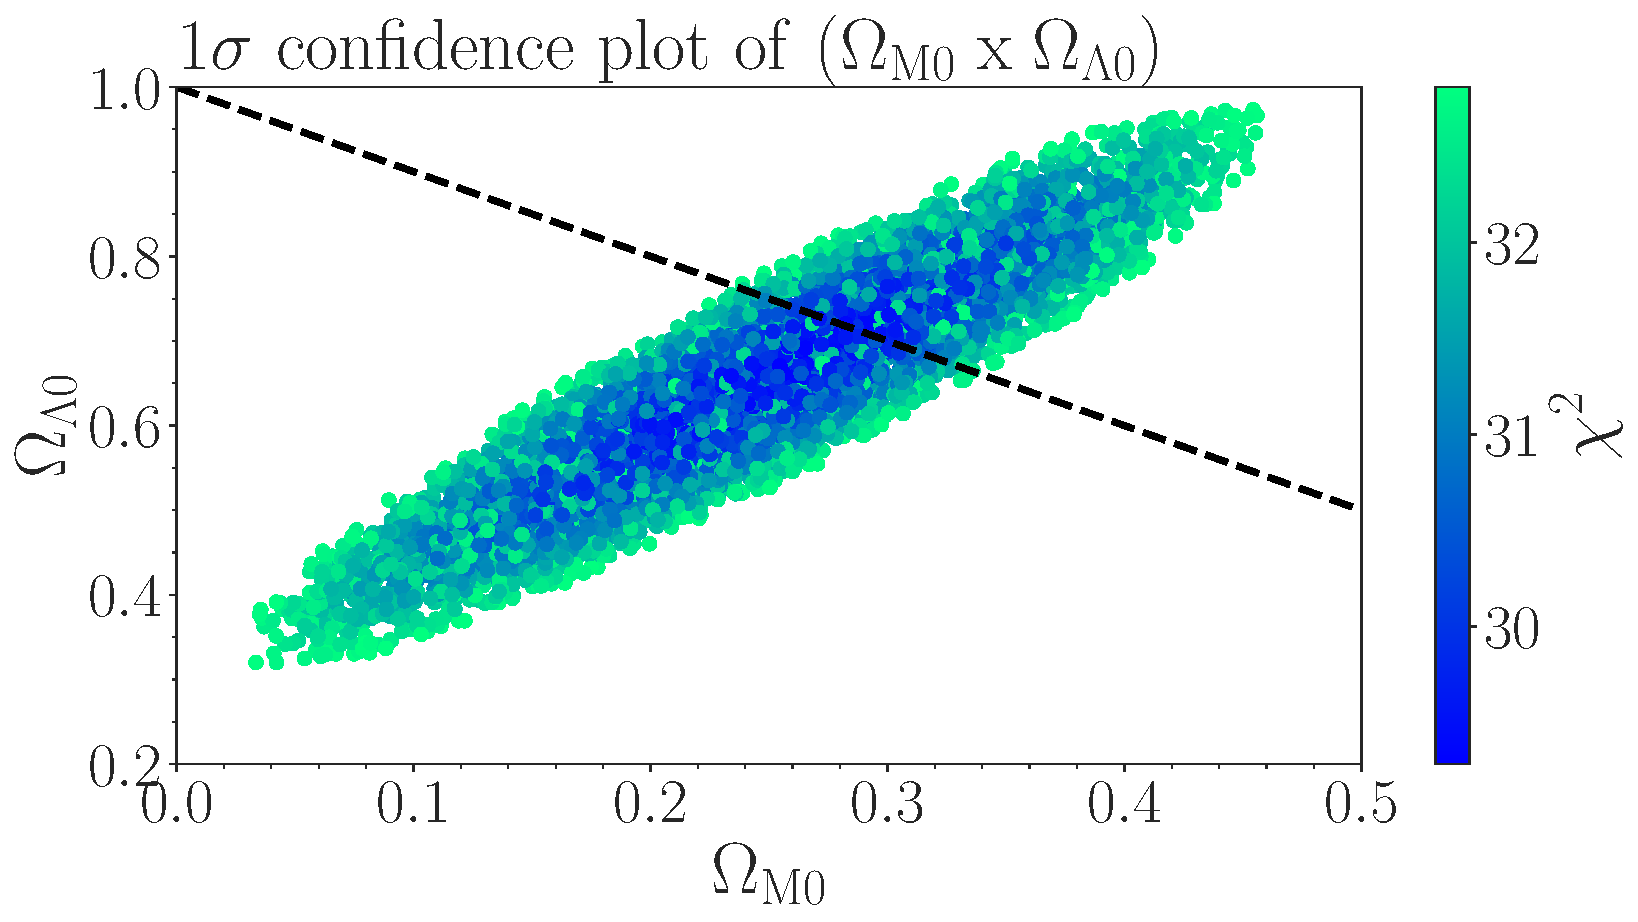
\includegraphics[width=\linewidth]{omega_plane.pdf}
        \caption{Scatter plot showing the $chi^2$-error of the luminosity distance $d_L$ between the observed values and the prediction, as function of $\O_\mathrm{M}$ and $\O_\Lambda$. The data shown is within $1\sigma$ (standard deviation). The black dotted line signifies a flat universe. }
        \label{fig:m1:omega_planes}
    \end{figure}

    The MCMC method allow us to make a posterior probability distribution of the parameters in question. \cref{fig:m1:posterior_pdf} the distribution of the Hubble factor $H_0$ constructed from the sampled values of $h$. The actual samples are shown in green and the corresponding fitted probability distribution in blue. 

    \begin{figure}
        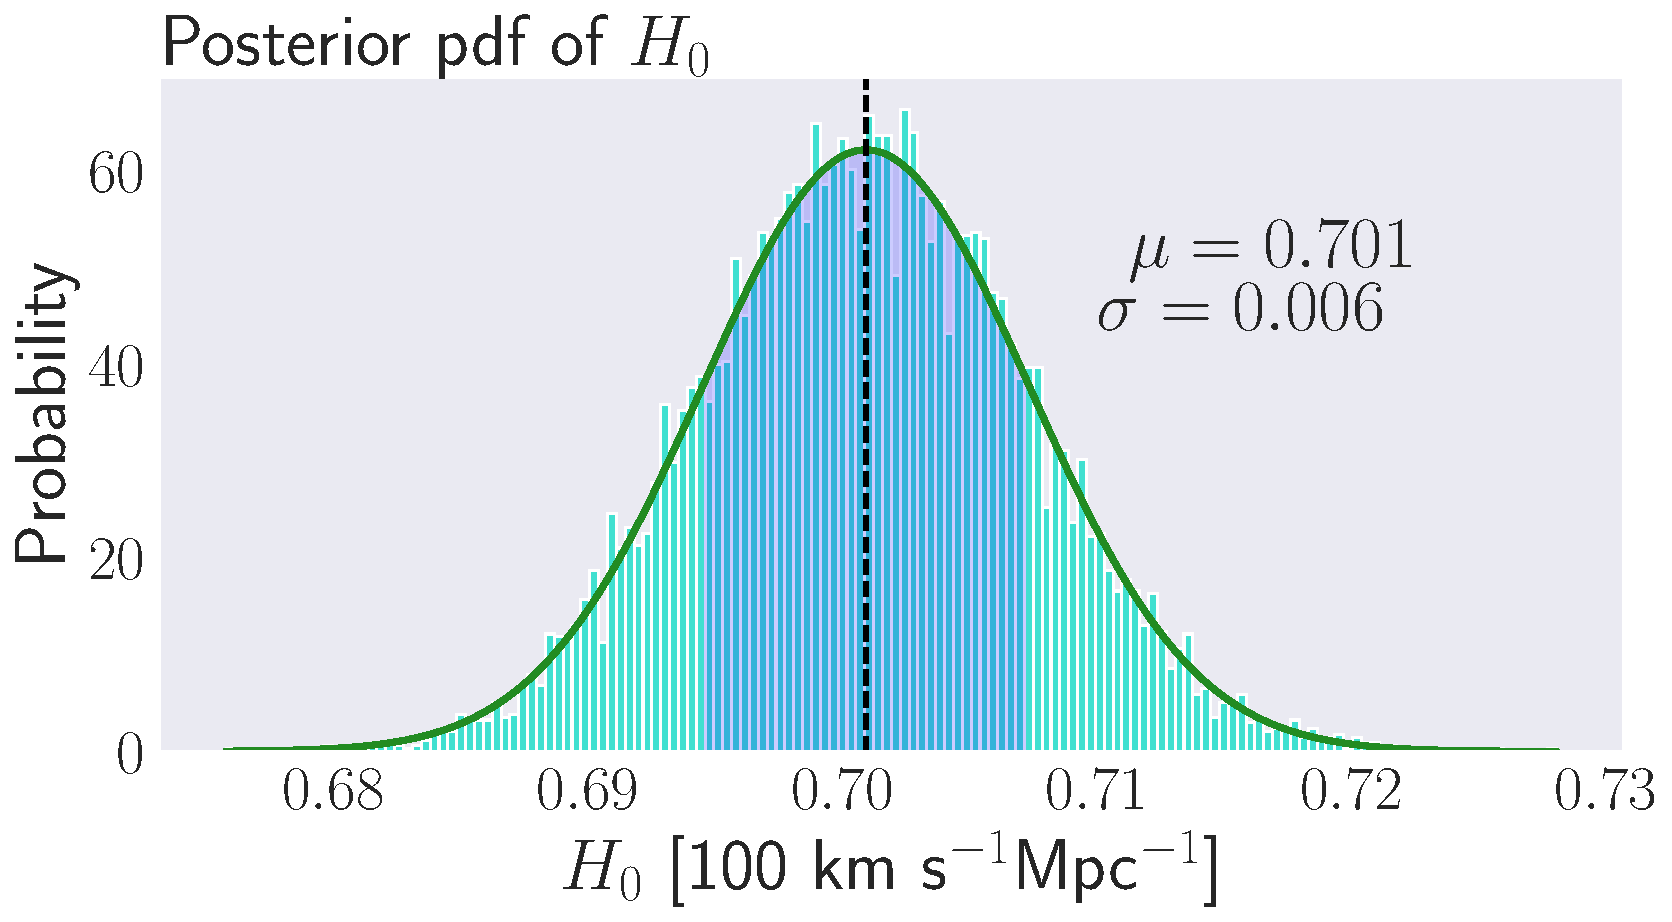
\includegraphics[width=\linewidth]{posterior_pdf.pdf}
        \caption{Posterior probability distribution (pdf) of $H_0$ as result of the MCMC sampling. The samples are shown in green, and the construction pdf in blue. }
        \label{fig:m1:posterior_pdf}
    \end{figure}

